\documentclass[a4paper, 12pt]{article}%тип документа

%отступы
\usepackage[left=2cm,right=2cm,top=2cm,bottom=3cm,bindingoffset=0cm]{geometry}
\setlength{\parindent}{5ex}

%Русский язык
\usepackage[T2A]{fontenc} %кодировка
\usepackage[utf8]{inputenc} %кодировка исходного кода
\usepackage[english,russian]{babel} %локализация и переносы

%Вставка картинок
\usepackage{graphicx}
\graphicspath{{pictures/}}
\DeclareGraphicsExtensions{.pdf,.png,.jpg}

%Графики
\usepackage{pgfplots}
\pgfplotsset{compat=1.9}

%Математика
\usepackage{amsmath, amsfonts, amssymb, amsthm, mathtools}

%Таблицы
\usepackage{longtable} 
\usepackage{float}

%Римские цифры
\newcommand{\RomanNumeralCaps}[1]{\uppercase\expandafter{\romannumeral#1}}

\usepackage{multirow}


\begin{document}
	\begin{titlepage}
		\begin{center}
			\textsc{Федеральное государственное автономное образовательное учреждение высшего образования«Московский физико-технический институт (национальный исследовательский университет)»\\[5mm]
			}
			
			\vfill
			
			\textbf{Отчёт по лабораторной работы 2.1.1\\[3mm]
				ИЗМЕРЕНИЕ УДЕЛЬНОЙ
				ТЕПЛОЁМКОСТИ ВОЗДУХА ПРИ
				ПОСТОЯННОМ ДАВЛЕНИИ.
				\\[50mm]
			}
			
		\end{center}
		
		\hfill
		\begin{minipage}{.5\textwidth}
			Выполнил студент:\\[2mm]
			Сериков Василий Романович\\[2mm]
			группа: Б03-102\\[5mm]
			
		\end{minipage}
		\vfill
		\begin{center}
			Москва, 2022 г.
		\end{center}
		
	\end{titlepage}
	
	\newpage
	\textbf{Аннотация}\\
	
	
	\textbf{Цель работы: }\\
	
	Измерить повышение температуры воздуха в зависимости от мощности подводимого тепла и расхода при стационарном течении через трубу; исключив тепловые потери, по результатам измерений определить теплоёмкость воздуха при постоянном давлении.\\
	
	
	\textbf{Теоретические сведения: } \\
	
	
	Измерение теплоёмкости тел обычно производится в калориметрах, т. е. в
	сосудах, обеспечивающих теплоизоляцию исследуемого тела от внешней
	среды. При этом регистрируется изменение его температуры $dT$ в зависимости от количества тепла $\delta Q$, полученного телом от некоторого нагревательного элемента внутри калориметра. Теплоёмкость тела в некотором процессе определяется как их отношение:
	\begin{align}
		C = \frac{\delta Q}{dT}.
	\end{align}
	Надёжность измерения определяется, в основном, качеством калориметра.
	Необходимо, чтобы количество тепла, затрачиваемое на нагревание исследуемого тела, существенно превосходило тепло, расходуемое на нагревание самого калориметра, а также на потери тепла из установки. При измерении теплоёмкости газов эти требования выполнить довольно трудно — масса газа в калориметре и, следовательно, количество тепла, идущее на его нагревание, как правило, малы. Для увеличения количества нагреваемого газа при неизменных размерах установки в нашей работе исследуемый газ (воздух) продувается через калориметр, внутри которого установлен нагреватель. При этом измеряются мощность нагревателя, масса воздуха, протекающего в единицу времени (расход), и приращение его температуры.
	
	Рассмотрим газ, протекающий стационарно слева направо через
	трубу постоянного сечения, в которой установлен нагревательный элемент. Пусть за некоторое
	время $dt$ через калориметр прошла малая порция газа массой $dm = q dt$, где $q$ --- массовый расход газа в трубе. Если мощность нагрева равна $N$, мощность тепловых потерь на обмен с окружающей средой $N_{\text{пот}}$, то порция получила тепло $\delta Q = (N - N_{\text{пот}})dt$. С другой стороны, по определению теплоёмкости $\delta Q = c dm \Delta T$, где $\Delta T = T_2 - T_1$ --- приращение температуры газа, $c$ --- удельная теплоёмкость газа в рассматриваемом процессе. При малых расходах газа и достаточно большом диаметре трубы перепад давления на её концах мал, потому можно принять, что $P_1 \approx P_2 = P_0$, где $P_0$ --- атмосферное давление. Следовательно, в условиях опыта измеряется удельная теплоёмкость при постоянном давлении $c_p$. Таким образом, получаем
	\begin{align}
		c_p = \frac{N - N_{\text{пот}}}{q \Delta T}
	\end{align}
	
	\textbf{\textit{Течение газа по трубе:}}
		В общем случае давление
	на входе может заметно превышать таковое на выходе
	(например, если труба достаточно узкая и длинная). Рассмотрим течение газа более
	детально, чтобы выяснить пределы применимости $P = const$. Обозначим индексом 1 параметры газа на входе в трубку, индексом 2 --- на выходе из неё. Рассмотрим область, мысленно ограниченную двумя неподвижными плоскостями слева и справа от нагревателя и применим к ней закон сохранения энергии.
	
	Пусть за время $dt$ газ сместился слева направо на малое расстояние вдоль
	трубки, такое что через левую границу прошёл газ объёмом $dV_1$m а через правую --- $dV_2$. В силу закона сохранения массы имеем
	\[
	m = \rho_1 dV_1 = \rho_2 d V_2,
	\]
	где $dm = q dt$ --- масса газа, прошедшего через некоторое сечение трубки.
	Изменение внутренней энергия газа в рассматриваемой области за счет переноса вещества составило $dU = (u_2 - u_1)dm$, где $u_{1, 2}$ --- удельные внутренние энергии. Внешние силы совершили работу по перемещению газа $\partial A = P_1 dV_1 - P2 dV_2$, или с учётом предыдущей формулы:
	\[
	\partial A = - (\frac{P_2}{\rho_2} - \frac{P_1}{\rho_1})dm.
	\]
	Учтем также изменение кинетической энергии течения газа, равное $dK = \frac{1}{2}(v_2^2 - v_1^2)dm$, где $v_{1, 2}$ --- скорости течения. Наконец, пусть $\partial Q$ --- количество тепла, суммарно полученное газом в рассматриваемой области --- включая тепло от нагревателя, теплопередачу через стенки и торцы, тепловыделение при трении и т. д. В стационарном состоянии энергия газа, заполняющего калориметр, неизменна, поэтому
	\[
	dU - dA + dK = \partial Q
	\]
	Полученное удобно записать в виде
	\[
	(i_2 - i_1 + \frac{v_2^2}{2} - \frac{v_1^2}{2}) dm = \partial Q,
	\]
	где $i = u + \frac{P}{\rho}$ --- удельная энтальпия газа.
	Это соотношение справедливо для любой стационарно текущей непрерывной среды и представляет собой обобщение известного уравнения Бернулли, учитывающее выделение и потери тепла. Оно справедливо при условии, что в системе устанавливается не только стационарное течение, но и стационарное распределение температуры. Последнее весьма важно для нашего опыта, поскольку время установления может быть довольно велико.
	
	Если предположить, что кинетическая энергия течения мала по сравнению с энергией нагрева ($dK \ll \partial Q$), то получим 
	\[
	(i_2 - i_1) dm = \partial Q,
	\]
	то есть полученное газом тепло идёт на приращение его энтальпии.
	
	В условиях опыта газ с хорошей точностью можно считать идеальным: $P / \rho = RT / \mu$, а теплоёмкость $c_p$ (или $c_v$) не зависящей от температуры. Тогда энальпия (и внутренняя энергия) газа зависит только от температуры и равна $\Delta i = c_p \Delta T$ (т. к. $\Delta u = c_V \Delta T$ и $c_p = c_v + \frac{R}{\mu}$).\\
	
	\newpage
\textbf{Методика измерений: }\\


\begin{figure}[h]
	\center{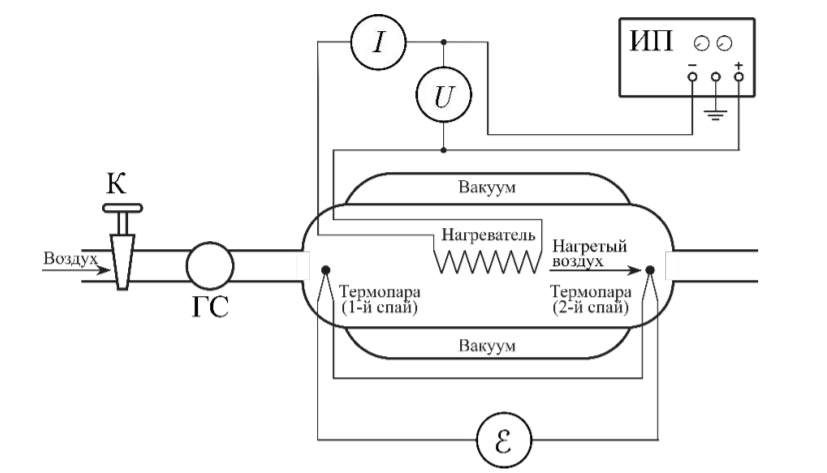
\includegraphics [scale=1]{installation.png}}
	\caption{Схема экспериментальной установки}
\end{figure}
Схема установки изображена на рис. 1. Воздух, нагнетаемый компрессором, прокачивается через калориметр. Калориметр представляет собой стеклянную цилиндрическую трубку с двойными стенками, запаянными с торцов. На внутреннюю поверхность стенок трубки нанесено серебряное покрытие для минимизации потерь тепла за счет излучения. Воздух из пространства между стенками калориметра откачан до высокого вакуума (10$^{-5}$ торр) для минимизации потерь тепла, обусловленных теплопроводностью. Нагреватель в виде намотанной на пенопласт нихромовой проволоки расположен внутри калориметра непосредственно в воздушном потоке. Нагрев проволоки производится от регулируемого источника постоянного тока (ИП). Напряжение $U$ на нагревателе и ток $I$ через него регистрируются цифровыми
мультиметрами. Таким образом, мощность нагрева равна
	\begin{align}
		N = UI.
	\end{align}
	
	Для измерения разности температур $\Delta T$ служит медно-константановая термопара. Один спай термопары расположен в струе воздуха, входящего в калориметр, и находится при комнатной температуре, а второй - в струе выходящего нагретого воздуха. Константановая проволока термопары расположена вдоль калориметра, а медные проводники подключены к цифровому вольтметру. Возникающая в термопаре ЭДС пропорциональна разности температур $\Delta T$ спаев:
	\[
	\mathcal{E} = \beta \Delta T,	
	\]
	где $\beta = 40.7 \frac{\text{мкВ}}{K}$ --- чувствительность медно-константановой термопары в рабочем диапазоне температур. ЭДС регистрируется с помощью микровольтметра.
	
	Объём воздуха, прошедшего через калориметр, измеряется газовым счётчиком ГС. Для регулировки служит кран K. Время $\Delta t$ прохождения некоторого объёма $\Delta V$ воздуха измеряется секундомером. Объёмный расход может быть найден как
	\[
	q = \rho \frac{\Delta V}{\Delta t},
	\]
	где $ \rho $ --- плотность воздуха при комнатной температуре, которая в свою очередь может быть получена из уравнения Менделеева-Клапейрона:
	\[
	\rho_0 = \frac{\mu P_0}{R T_0},
	\]
	где $P_0$ --- атмосферное давление, $T_0$ --- комнатная температура (в Кельвинах), $\mu = 29,0 \frac{\text{г}}{\text{моль}}$ --- средняя молярная масса (сухого) воздуха.
	
	Учитывая особенности калориметра, следует ожидать, что мощность нагревателя расходуется не только на нагрев массы прокачиваемого воздуха, но и частично теряется за счёт нагрева внутренних стенок термостата и рассеяния тепла через торцы термостата. Можно предположить, что при небольшом нагреве $(\Delta T \ll T_0)$ мощность потерь тепла $N_{\text{пот}}$ прямо пропорциональна разности температур:
	\[
	N_{\text{пот}}=\alpha\ \Delta T
	\]
	Следовательно, при фиксированном расходе воздуха $(q = const)$ подводимая мощность и разность температур связаны прямой пропорциональностью $\left( \Delta T (N) \right)$ --- линейная функция).
	\[
	N = (c_Pq+\alpha)\Delta T
	\]\\
	
	
	\textbf{Используемое оборудование: }\\
	
	
	Теплоизолированная стеклянная трубка; электронагреватель; источник питания постоянного тока; амперметр, вольтметр (цифровые мультиметры); термопара, подключенная к микровольтметру; компрессор; газовый счётчик;
	секундомер.\\
	
	
	\textbf{Результаты измерений и обработка данных: }\\
	\begin{enumerate}
		\item Запишем начальные данные: $t_0 = 20,7^{\circ}C$ -- температура в кабинете, $P_0 = 102,05$ кП -- давление, $\phi_0 = 15,3 \% $ -- влажность, $R$ = 35 Ом -- сопротивление проволоки. $\sigma_V = \pm 0,01$л, $\sigma_{\Delta t} = 0,1$ с, $\sigma_{\varepsilon} = \pm 1 \cdot 10^{-6} $В, $\sigma_U = \pm 0,01$ В, $\sigma_I = \pm 1 \cdot 10^{-5}$ А
		
		\item С помощью газового счетчика и секундомера измерим максимальный расход воздуха, определим среднее значение и вычислим массовый расход. Данные занесем в таблицу.

\newpage

\begin{longtable}{|c|c|c|}
	\hline
	$ \Delta V, $л & $ \Delta t $, с & $ q $, л/с  \\ \hline
	1 & 5,2 & 0,192  \\ \hline
	2 & 9,8& 0, 204 \\ \hline
	3 & 15,2 & 0,197 \\ \hline
	4 & 20,3 & 0,197 \\ \hline
	5 &  25,3 & 0,197 \\ \hline
	\multicolumn{3}{|c|}{$q_{max} = 0,197 \pm 0,003$ л/с}  \\ \hline
	\multicolumn{3}{|c|}{$q_{max}^{\text{масс}} = 0, 236 \pm 0,006$ г/с}  \\ \hline
	\caption{Результаты вычислений для $q_{max}$ и $q_{max}^{\text{масс}}$.}
\end{longtable}

	\item Оценим  величину тока нагревателя $I_0$ требуемого для нагрева воздуха на $\Delta T_0 = 1^{\circ}C$. Для этого оценим минимальную мощность  $N_0$ , необходимую для нагрева газа при максимальном расходе $q_{max}$ на $\Delta T_0 = 1^{\circ}C$, тогда $I_0 = \sqrt {\frac{N_0}{R}}$

	$$N_{0} = c_{p}q\Delta T  = (0, 236 \pm 0,006)\text{Вт}  => I_0 = (0, 082 \pm 0,002) \text{А}$$
	
	\item . Проведем измерение зависимости разности температур от мощности
	нагрева $T(N)$ при максимальном расходе воздуха. Данные занесем в таблицу.
	
\begin{longtable}{|c|c|c|c|c|c|}
	\hline
	$I, $мА & $U, $В &$\varepsilon, $мВ & $ \Delta T, $К & $N, $Вт &  $R, $Ом 
	\\
	\hline
	82,5 & 2,91 & 0.34 & 0.835 & 0,239 &  35,15
	\\
	\hline
	116,1 & 4,14 & 0.68 & 1,67 & 0,476 & 35,31
	\\
	\hline
	145,3 & 5,18 & 0.106 & 2,60 & 0,741 & 35,1
	\\
	\hline
	165,4 & 5,82 & 0.140 & 3,44 & 0,959 & 35,06
	\\
	\hline
	\caption{Измерение $\Delta T (N)$ для $ q_{max}$}
\end{longtable}

	\item Повторим пункты 1-4 для 2-х других значений $q$. Получим Результаты вычислений для $q_i$ и $q_i^{\text{масс}}$, $i = 1, 2$

	\begin{minipage}{0.4\textwidth}
\begin{longtable}{|c|c|c|}
	\hline
	$ \Delta V, $л & $ \Delta t $, с & $ q $, л/с  \\ \hline
	1 & 5,4 & 0,183  \\ \hline
	2 & 10,8& 0, 184 \\ \hline
	3 & 15,9 & 0,188 \\ \hline
	4 & 21,3 & 0,187 \\ \hline
	5 &  26,5 & 0,188 \\ \hline
	\multicolumn{3}{|c|}{$q_1 = 0,186 \pm 0,003$ л/с}  \\ \hline
	\multicolumn{3}{|c|}{$q_1^{\text{масс}} = 0, 223 \pm 0,005$ г/с}  \\ \hline
\end{longtable}
\end{minipage} 
\begin{minipage}{0.4\textwidth}
	\begin{longtable}{|c|c|c|}
		\hline
		$ \Delta V, $л & $ \Delta t $, с & $ q $, л/с  \\ \hline
		1 & 5,9 & 0,167  \\ \hline
		2 & 11,6& 0,171 \\ \hline
		3 & 17,9 & 0,167 \\ \hline
		4 & 23,6 & 0,169 \\ \hline
		5 &  259,6 & 0,168 \\ \hline
		\multicolumn{3}{|c|}{$q_2 = 0,168 \pm 0,003$ л/с}  \\ \hline
		\multicolumn{3}{|c|}{$q_2^{\text{масс}} = 0, 202 \pm 0,005$ г/с}  \\ \hline
	\end{longtable}
\end{minipage} \\

	
	\newpage
	
\begin{longtable}{|c|c|c|c|c|c|}
	\hline
	$I, $мА & $U, $В &$\varepsilon, $мВ & $ \Delta T, $К & $N, $Вт &  $R, $Ом 
	\\
	\hline
	81,2 & 2,86 & 0.33 & 0.81 & 0,232 & 35,22
	\\
	\hline
	112,2 & 3,94 & 0.65 & 1,6 & 0,442 & 35,11
	\\
	\hline
	139,7 & 4,91 & 0.102 & 2,5 & 0,686 & 35,14
	\\
	\hline
	160,7 & 5,65 & 0.137 & 3,36 & 0,907 & 35,15
	\\
	\hline
\caption{Измерение $\Delta T (N)$ для $ q_1$}
\end{longtable}

\begin{longtable}{|c|c|c|c|c|c|}
	\hline
	$I, $мА & $U, $В &$\varepsilon, $мВ & $ \Delta T, $К & $N, $Вт &  $R, $Ом 
	\\
	\hline
	78 & 2,76 & 0.31 & 0.76 & 0,215 & 35,38 
	\\
	\hline
	109,7 & 3,88 & 0.65 & 1,6 & 0,425 & 35,36
	\\
	\hline
	129 & 4,55 & 0.093 & 2,28 & 0,587 & 35,27
	\\
	\hline
	149,8 & 5,29 & 0.128 & 3,14 & 0,792 & 35,31
	\\
	\hline
	\caption{Измерение $\Delta T (N)$ для $ q_2$}
\end{longtable}

	\item Построим графики зависимости $\Delta T (N)$ для каждого расхода q, найдем угловые коэффициенты, полученных прямых.

	\begin{figure}[h]
		\center{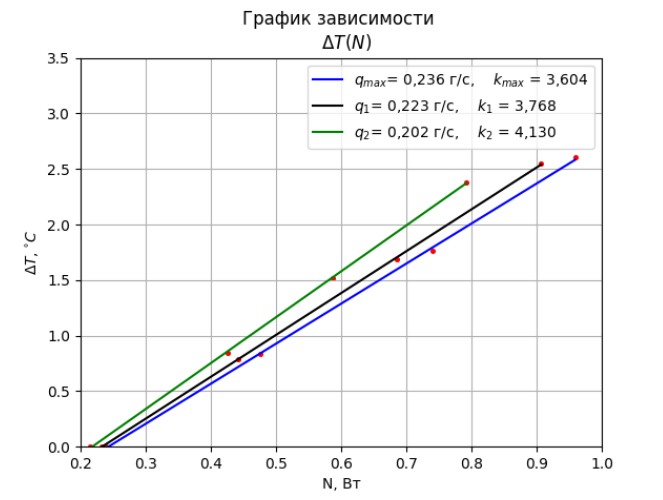
\includegraphics [scale=1]{Delta_T(N).png}}
	\end{figure}
	
\newpage
	\item Построим график зависимости $1/k(q)$ и по наклону прямой определим теплоёмкость воздуха $c_p$
	
	\begin{figure}[h]
		\center{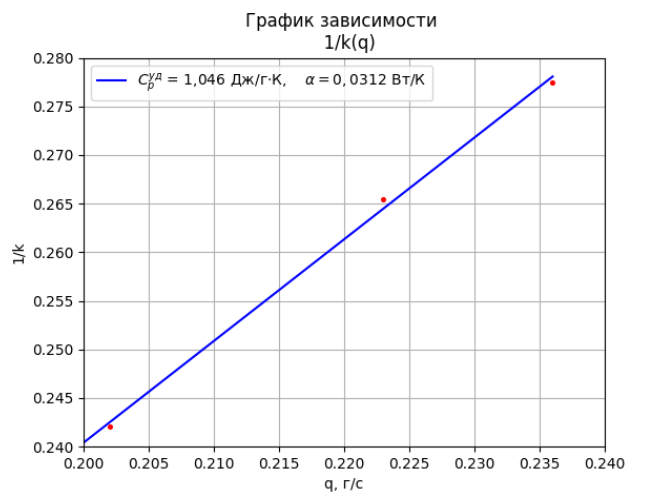
\includegraphics [scale=1]{1_k(q).png}}
	\end{figure}
	
	\item Таким образом $C_p = 30 \pm 1$ Дж/К$\cdot$моль
	\item Определим доли тепловых потерь: $\frac{N_{\text{пот}}}{N} =\alpha \cdot k$
	\begin{longtable}{|c|c|}
	\hline
	$q,$ г/с & $\frac{N_{\text{пот}}}{N}$ \\
	\hline
	0,236 & $0,11 \pm 0.01$ \\
	\hline
    0,223 & $0,12 \pm 0.01$\\
	\hline
    0,202 & $0,129 \pm 0.014$ \\
	\hline
	\end{longtable}
\end{enumerate}
	\textbf{Обсуждение результатов: }\\
	Мы определили молярную теплоемкость воздуха при постоянном давлении, которая составляет  $C_p = 30 \pm 1$ Дж/К$\cdot$моль, что в пределах погрешности совпадает с табличным значением ($C_p = 29,2$ Дж/К$\cdot$моль). Также мы оценили с хорошей точностью отношения $\frac{N_{\text{пот}}}{N}$ ($\varepsilon \approx 10 \% $ ).\\
	
	
	\textbf{Выводы: }\\
	В ходе данной работы мы измерили повышение температуры воздуха в зависимости от мощности подводимого тепла и расхода при стационарном течении через трубу; исключили тепловые потери и по результатам измерений определили теплоёмкость воздуха при постоянном давлении.
	
\end{document}